\usepackage[utf8]{inputenc}
\usepackage[T1]{fontenc}
\usepackage[french]{babel}
\usepackage{fancyhdr}
\usepackage{graphicx}
\usepackage{hyperref}
\usepackage{fontawesome}
\usepackage[left=3cm,right=3cm,top=4cm,bottom=4cm,textheight=28cm]{geometry}
\usepackage{wrapfig}
\usepackage{eso-pic}
\usepackage{transparent}
\usepackage{setspace}
\usepackage{titletoc}
\usepackage{enumerate}
\usepackage{titlesec}
\usepackage{xcolor}
\usepackage{listings}

\usepackage{lmodern}	% font definition
\usepackage{amsmath}	% math fonts
\newcommand{\Mod}[1]{\ (\mathrm{mod}\ #1)}

\usepackage{amsthm}
\usepackage{amsfonts}
\usepackage{mathrsfs}

\usepackage{pgfplots}
\usepackage{tikz}
\usetikzlibrary{matrix,chains,positioning,decorations.pathreplacing,arrows}


\newcommand\BackgroundPic{%
	\put(0,-50){%
		\parbox[b][\paperheight]{\paperwidth}{%
			%\vfill
			\centering
			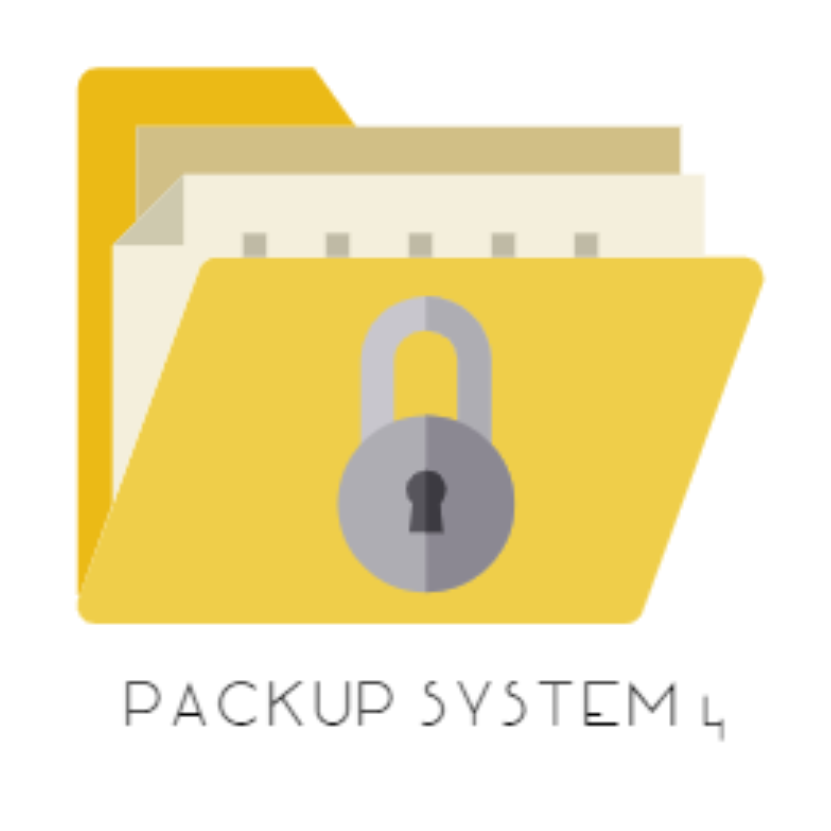
\includegraphics[scale=0.30]{./images/ps4logo-min.png}%
			\vfill
		}
	}
}

\renewcommand{\baselinestretch}{1.4}

\titleformat{\section}[block]{\Large\bfseries\filcenter}{\thesection}{1em}{}

\definecolor{mGreen}{rgb}{0,0.6,0}
\definecolor{mGray}{rgb}{0.5,0.5,0.5}
\definecolor{mPurple}{rgb}{0.58,0,0.82}
\definecolor{backgroundColour}{rgb}{0.95,0.95,0.92}

\lstdefinestyle{CStyle}{
    backgroundcolor=\color{backgroundColour},   
    commentstyle=\color{mGreen},
    keywordstyle=\color{magenta},
    numberstyle=\tiny\color{mGray},
    stringstyle=\color{mPurple},
    basicstyle=\footnotesize,
    breakatwhitespace=false,         
    breaklines=true,                 
    captionpos=b,                    
    keepspaces=true,                 
    numbers=left,                    
    numbersep=5pt,                  
    showspaces=false,                
    showstringspaces=false,
    showtabs=false,                  
    tabsize=2,
    language=C
}

\lstdefinestyle{CStyleSmall}{
    backgroundcolor=\color{backgroundColour},   
    commentstyle=\color{mGreen},
    keywordstyle=\color{magenta},
    numberstyle=\tiny\color{mGray},
    stringstyle=\color{mPurple},
    basicstyle=\tiny,
    breakatwhitespace=false,         
    breaklines=true,                 
    captionpos=b,                    
    keepspaces=true,                 
    numbers=left,                    
    numbersep=5pt,                  
    showspaces=false,                
    showstringspaces=false,
    showtabs=false,                  
    tabsize=2,
    language=C
}

\title{\textbf{{\Huge Rapport de Projet}}}
\author{
	\\
	\bsc{{\LARGE \bf Packup System 4}} \\ \\ \\
	\bsc{MAUBANC "Hyperion" Rémi} \\
	\bsc{RIDEAU "Pokkihju" Cyril} \\
	\bsc{CASIER "Zaihner" Frédéric} \\
	\bsc{FARINAZZO "KernelKiller" Cédric} \\ \\ \\
}
\date{{\LARGE \today}}

\pagestyle{fancy}
\fancyfoot[L]{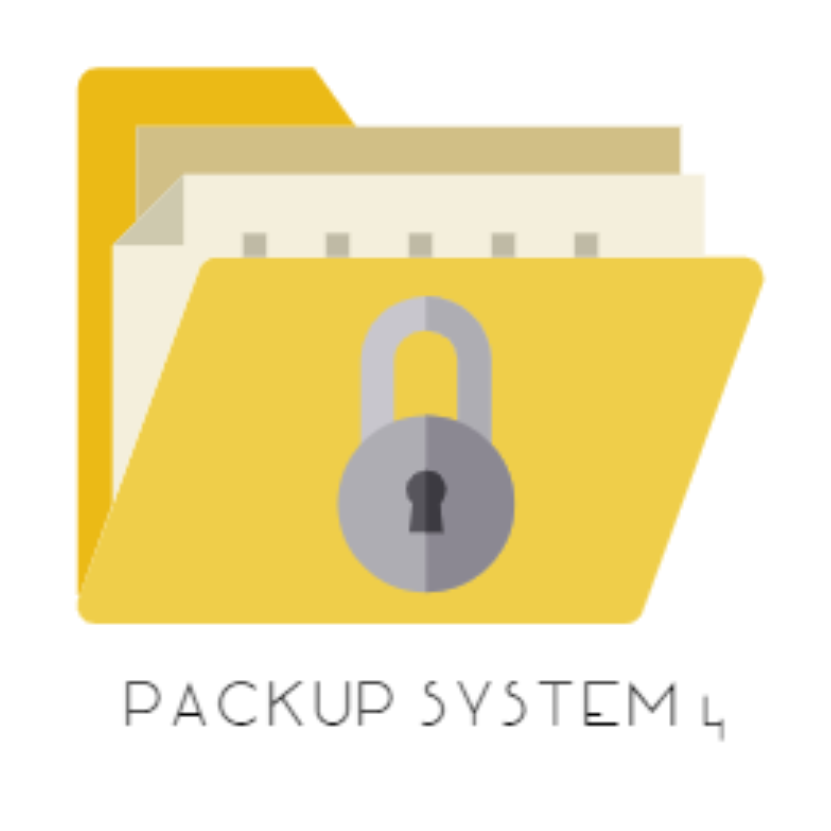
\includegraphics[scale=0.05]{./images/ps4logo-min.png}}
\fancyfoot[R]{EPITA 2022}
\fancyhead[R]{PS4}
\fancyhead[L]{Rapport de Projet}

\setcounter{tocdepth}{5}